\documentclass{article}
\usepackage{amsmath}
\usepackage{mathtools}
\usepackage{amsfonts}
\usepackage{amssymb}
\usepackage{amsthm}
\usepackage{fancyhdr}
\usepackage{float}
\usepackage{epigraph}
\usepackage{caption}
\usepackage{esint}

%Page formatting
\lhead{Eric Du}
\chead{Homework 5}
\rhead{\today}
\pagestyle{fancy}
\cfoot{\thepage}
\title{Homework 5}
\author{Eric Du}
\date{\today}

%.sty file handling
\usepackage[sexy]{evan}
\usepackage{tcolorbox}
\usepackage{xcolor}
\renewcommand{\labelitemi}{\textendash}
\renewcommand{\abstractname}{}
\theoremstyle{definition}
\newtheorem*{solution}{\color{blue}Solution}
\numberwithin{equation}{section}
\numberwithin{definition}{section}

%Paragraph Formatting
\setlength{\epigraphwidth}{148pt}
\setlength{\parindent}{0pt}
\linespread{1.3}
\allowdisplaybreaks

%TikZ special settings
\usepackage{circuitikz}
\usetikzlibrary{shapes.geometric}
\usetikzlibrary{decorations.markings}

\begin{document}
\maketitle
\begin{abstract}
    \textbf{[NOTE:]} to complete this homework I worked together with \textbf{Andrew Binder}. Credit also goes to Andrew for supplying me with his Ti\textit{k}Z diagrams.
\end{abstract}

\section{Problem 1}

\subsection{Part a}
\label{q1a}
From the diagram: 

$$\begin{tikzpicture}
    \draw[thick] (-3,-1) -- (3,-1);
    \draw (-1,0) -- (1,0) -- (1,2) node[midway, right, color=purple] {$a$} -- (-1,2) node[midway, above, color=purple] {$a$} -- cycle;
    \draw[-stealth] (-2.5,-0.55) -- (-1,-0.55) node[midway, below] {$I'$};
    \draw[stealth-stealth, color=purple] (0,-1) -- (0,0) node[midway, right] {$s$};
    \draw[-stealth] (-1.25,1.5) -- (-1.25,2.25) node[midway, left] {$I$} -- (-0.75,2.25);
  \end{tikzpicture}$$

Note that the only contributions to force are where the direction of the current is parallel or antiparallel to infinitely long wire. This is because for the sides which are parallel to the vertical direction, the forces exactly cancel. For a section of the loop of length $a$, we have:

\[ F_{loop} = I a B_{wire}\]

This formula is specifically for two wires whose directions are parallel to one another. From Ampere's law, we have $B_{wire} = \dfrac{\mu_0 I'}{2\pi r}$, where $r$ represents the distance between the two wires in question. Since these two sections of the loop are at different distances, we need to add them them up separately. Doing so, we obtain:

\begin{align*}
    \sum F &= Ia \frac{\mu_0I'}{2\pi s}\hat \jmath  - Ia\frac{\mu_0I'}{2\pi (s+a)}\hat \jmath\\
    &= \frac{Ia\mu_0I'}{2\pi}\left(\frac{1}{s} - \frac{1}{s+a}\right)\hat \jmath
\end{align*}

Note that in this problem we've chosen the positive direction to point upwards, so the net force in this case, since $\dfrac{1}{s} - \dfrac{1}{s+a} > 0$, would be pointing upwards. 

This result makes sense, since we expect the contribution of force from the wire segment closer to the long wire to have a much stronger contribution, so we expect the net force to not be zero. Additionally, we expect the net force to point upwards due to the right hand rule.

\begin{remark}
  Note that the force formula we use here $F = IaB_{wire}$ is inherently assuming that both wires are parallel with one another. This is not true in the case of part b (as will become evident with the non-parallel sides).
\end{remark}
\subsection{Part b}

Again, refer to the diagram below:

$$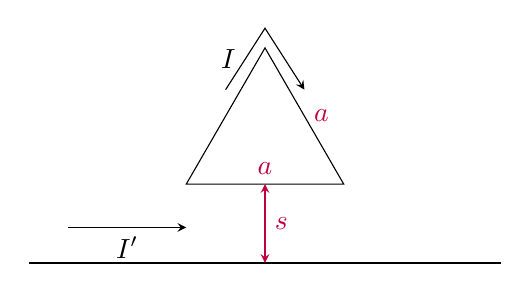
\begin{tikzpicture}
    \draw[thick] (-3,-1) -- (3,-1);
    \draw (-1,0) -- (1,0) node[midway, above, color=purple] {$a$} -- (0,1.73) node[midway, right, color=purple] {$a$} -- cycle;
    \draw[-stealth] (-2.5,-0.55) -- (-1,-0.55) node[midway, below] {$I'$};
    \draw[stealth-stealth, color=purple] (0,-1) -- (0,0) node[midway, right] {$s$};
    \draw[-stealth] (-0.5, 1.2) -- (0,1.98) node[midway, left] {$I$} -- (0.5, 1.2);
  \end{tikzpicture}$$

We still use the following formula:

\[ F = I a B_1\]

Where $B_1$ denotes the magnetic field contributions from the long wire. The force from the wire segment parallel is the same as that from section \ref{q1a}, which will be:

\[ F_1 = \frac{\mu_0 IaI'}{2\pi s}\]

For the other two non-parallel sides, the current vector and the $\vec{B}$ field are at right angles to one another. By the right hand rule, we find that the forces from these sections are going to be pointing as follows:

% Insert diagram here

Notice then that the $\hat \imath$ components of these two forces will cancel, so all that remains is the $\hat \jmath$ components. So we can solve for the force and only take the $\sin \alpha$ component of that force. From geometry, we know that $\alpha = 30^\circ$, so all we really need to do is halve the total force we find.

\begin{align*}
  \vec F &= q \vec v \times \vec B \\
  \therefore dF &= dq \vec v \times \vec B\\
  &= I \vec dl \times \vec B
\end{align*}

We already know that $B(r) = \dfrac{\mu_0 I}{2\pi y}$, where $y$ denotes the distance from the infinitely long wire to a segment on the loop. Thus, in our case we essentially have to solve:

\begin{align*}
  \vec F_2 \sin \alpha &= \frac{1}{2} \int I dl \times \frac{\mu_0 I'}{2\pi y}\\
  &= \frac{1}{2} \frac{\mu_0 II'}{2\pi}\int dl \frac{1}{y}\\
\end{align*}

Now consider a segment $dl$. Notice that we can actually write $dy = dl \sin 60^\circ$, and thus $dl = \dfrac{2dy}{\sqrt{3}}$. From here, we can also plug in the bounds to be integrating from a y-coordinate of $s$ to $s + \dfrac{a\sqrt{3}}{2}$.

\begin{align*}
  |\vec{F}| &= \frac{\mu_0 II'}{2\sqrt{3}\pi} \int_s^{\frac{\sqrt{3}a}{2} + s} \frac{1}{y} dy\\
  &= \frac{\mu_0 II'}{2\sqrt{3}\pi} \left[\ln\left(\frac{\sqrt{3}a}{2} + s\right) - \ln s\right]\\
  &= \frac{\mu_0 II'}{2\sqrt{3}\pi} \ln \left(\frac{\sqrt{3}a}{2s} + 1\right)
\end{align*}

Notice that there are also two segments of the wire, so we need to double this force. Moreover, due to the right hand rule this force points downward, so we finally get:

\[ \vec{F} = -\frac{\mu_0 II'}{\sqrt{3}\pi}\ln\left(\frac{\sqrt 3 a}{2s} + 1\right) \hat \jmath\]

Thus, the net force on the total system:

\begin{align*}
  \sum F &= \frac{\mu_0 aII'}{2\pi s}\hat \jmath - \frac{\mu_0 I^2}{\sqrt{3}\pi}\ln\left(\frac{\sqrt 3 a}{2s}+ 1\right) \hat \jmath\\
  &=\frac{\mu_0 I I'}{\pi}\left[\frac{1}{2s} - \frac{1}{\sqrt{3}}\ln\left(\frac{\sqrt{3}a}{2s}+ 1\right)\right]
\end{align*}

\section{Problem 2}

Refer to the following diagram: 

$$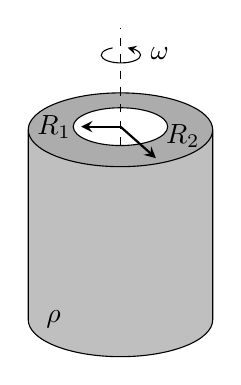
\begin{tikzpicture}
    \node[cylinder,
            draw = black,
            text = black,
            cylinder uses custom fill,
            cylinder body fill = gray!50,
            cylinder end fill = gray!65,
            aspect = 0.4,
            scale=10,
            shape border rotate = 90] (c) at (0,0) {};
    \node at (-0.85,-0.7) (r) {$\rho$};
    \draw[black, fill=white] (0,1.75) ellipse (0.6cm and 0.24cm);
    \draw[dashed] (0,1.51) -- (0,3);
    \draw[-stealth, thick] (0,1.75) -- (-0.5,1.75) node[anchor=east] {$R_1$};
    \draw[-stealth, thick] (0,1.75) -- (0.45,1.35) node[anchor=south west] {$R_2$};
    \draw[-{stealth[scale=0.5]}] (-0.1,2.75) arc
      [
          start angle=115,
          end angle=430,
          x radius=0.25cm,
          y radius =0.1cm
      ] ;
    \node at (0.5,2.675) (w) {$\omega$};
\end{tikzpicture}$$


\subsection{Part a}
\label{q2a}

Take a closed loop whose vertical segments are outside the wire and inside the hole of the cylinder. We know that the $\vec{B}$ field outside the cylinder is zero (this will be shown to be true in part c), so the only nonzero contribution from our $\vec{B}$ field would be from the segment within the loop. Let's consider this vertical segment within the loop to have height $L_1$, which will cancel later on in the calculation. Thus, we have $\mu_0 I_{enc} = BL_1$. Now, computing $I_{enc}$:

\begin{align*}
  I &= \frac{dq}{dt}\\
  dq &= \rho dV\\
  &= \rho A (R_2 - R_1) d\theta\\
  \therefore I &= \frac{\rho A (R_2 - R_1) d\theta}{dt}
\end{align*}

Notice that $\dfrac{d\theta}{dt} = \omega$, so simplifying this and quantifying $A$, we get:

\begin{align*}
  I &= (R_2 - R_1) \rho (R_2 - R_1)L_1 \omega\\
  &= (R_2 - R_1)^2 \rho L_1 \omega
\end{align*}

So finally, we have: 

\begin{align*}
  BL_1 &= \mu_0 \rho L_1 \omega (R_2 - R_1)^2\\
  \therefore B &= \mu_0 \rho \omega(R_2 - R_1)^2 
\end{align*}

This means that the $\vec{B}$ field is constant within the cylinder. This result makes sense, since we would expect that this system, which is very similar to a solenoid, should produce very similar results. Furthermore, by Ampere's law, the depth we choose for our amperian loop does not change the enclosed current (as long as the vertical segment located within the cylinder remains there), so we should expect that the $B$ field is constant inside from that calculation as well.


\subsection{Part b}

For this problem we choose different loops at varying depths to the rotating cylinder. Just like the previous problem, we have $\mu_0 I_{enc} = BL_1$ for a loop of height $L_1$, and we compute $I_{enc}$ the same way except this time we substitute $R_1 = r$. Aside from this substitution, the algebra is exactly the same as the previous problem, so I won't repeat it here. At the end, we get:

\[ B(r) = \mu_0 \rho \omega (R_2 - r)^2 \]

\subsection{Part c}

For any point outside the cylinder, we can draw a closed rectangular loop just like the one we did in class with the solenoid. Computing ampere's law:

\[ \oint B dr = \vec{B}(r_1)L_1 + \vec{B}(r_2)L_1 = \mu_0 I_{enc}\]

And since $I_{enc} = 0$ and neither $r_1$ or $L_1$ can be zero, then this must imply that $\boxed{B = 0}$ outside the cylinder.

\section{Problem 3}

For this problem, we can essentially do the same as problem 2, but with different amperian loops.

\subsection*{Inside and outside the donut}

We pick an amperian loop just like the one we choose from part a) of problem 2 (found in section \ref{q2a}). However, we notice that due to the way the current travels around the solenoid, the current through the loop is zero. Thus, we get the following:

\[ \oint B dr = B(r_1) L_1 + B(r_2)L_1 = 0\]

This equation implies that $B(r_1) = - B(r_2)$. This is impossible, since we expect the $B$ field to form closed loops. As a result, the only resolution for this is if $B(r_1) = B(r_2) = 0$.

This means that the $B$ field both inside and outside the donut are both zero.

\subsection*{Inside the donut itself}

Here we choose an amperian loop which goes around the donut at a constant radius from its center. We have the following integral:

\[ \oint B dr = \mu_0 I_{enc}\]

We know that the $B$ field is constant because for any point on a circular loop, the solenoid looks identical, so the $B$ field must be the same by this argument. This is actually important, because it means that we can pull $B$ out of the integral, and now we can compute the path integral. Thus, we have:

\[B \cdot 2\pi r = \mu_0I_{enc}\]

We also know that $I_{enc} = 2\pi anI$ Therefore, we can write:

\begin{align*}
  B \cdot 2\pi r &= \mu_0 2\pi an I \\
  \therefore B &= \frac{\mu_0 naI}{r}
\end{align*}

The fact that $B$ here is a function of $r$ makes complete sense because when we integrate our amperian loop we are computing $\int B dl$, the size of our loop depends on $r$, whereas the enclosed current does not depend on $r$, so we should expect our $B$ field to depend on $r$.

\section{Problem 4}

We can essentially treat this system as two wires superimposed inside one another, with equal current going in opposite directions so as to create a ``hole'' with no current going through it.

The first step, as indicated by the hint, is to find the magnetic field inside a solid cylinder. We can do this by choosing a circular amperian loop, centered at the center of the cylinder, having arbitrary radius $r$:

\[\int B dl = \mu_0 I_{enc}\]

Note that for any location along this loop, we must have that the $B$ field is constant, since everywhere on the loop there is cylindrical symmetry. As a result, we can pull the $B$ outside of the integral, so our expression becomes:

\[ B 2\pi r = \mu_0 J \cdot \pi r^2\]

Where $J$ denotes the current density. The current density is equal to the current over the total cross-sectional area, so $J = \dfrac{I}{\pi R^2}$. But since the current density is constant throughout the wire, we also have: 

\begin{align*}
  J &= \frac{I_{tot}}{\pi R^2} = \frac{I_{enc}}{\pi r^2}\\
  \therefore I_{enc} &= \frac{r^2 I_{tot}}{R^2}
\end{align*}

Thus since $B \cdot 2\pi r = \mu_0 I_{enc}$, then we have:

\[ B = \frac{\mu_0 r I_{tot}}{2\pi R^2}\]

Since the $B$ field points in the direction of $\hat z \times \hat r = \hat \phi$, we get:

\[ B = \frac{\mu_0 rI_{tot}}{2\pi R^2} \hat \phi\]

Now we can use the law of superposition. First, we treat the outer cylinder to have a current going into the page, and the inner cylinder to have the same current density (this is the only way to guarantee $B$ field that perfectly counteracts the one made by the initial wire) but going \textit{out of the page}. Now we choose any point inside the hole, and call its distance from the point to the center of the large cylinder $R'$ and the smaller one $r'$:

\begin{align*}
  B_{tot} &= \frac{\mu_0 R' I_{tot}}{2\pi R^2} \hat \phi - \frac{\mu_0 r' I_{tot}}{2\pi R^2} \hat \phi\\
  &= \frac{\mu_0 I_{tot}}{2\pi R^2}(R' - r') \hat \phi
\end{align*}

Now notice that $R' - r'$ is constant (and so are the other terms), so as a result the $B$ field within the hole is constant in both magnitude and direction, which is what we wanted to show.

\section{Problem 5}

\subsection{Part a}

At the point $P_1$ the magneitc field strength is the same as that of a solenoid with $n$ turns, so its strength is: 

\[ B_1 = \mu_0 n I\]

The most important thing to note about this is the fact that this value is less than the $B$ field of a completely infinite solenoid (this is shown to be true in the textbook in figure 6.17). Now, we consider two semi-infinite solenoids joined end to end at $P_2$. By joining the two, we've essentially created an infinite solenoid, and thus the $B$ field at $P_2$ is now that of the infinite case. Thus, the $B$ field contribution at $P_2$ is half that of the $B$ field in the infinite case.

And since the $B$ field of an infinite solenoid is higher than that at the center of a finite one, we should expect that the $B$ field at $P_2$ is slightly more than half of the $B$ field at $P_1$.

\subsection{Part b}

We again use the argument of connecting two semi-infinite solenoids together with the same winding. When we join the two solenoids, we should expect an infinitely long solenoid in all directions, meaning that the $B$ field outside the solenoid must be zero (since there isn't any place for the $B$ field lines to ``escape" the inside solenoid). 

Furthermore, we should expect at the junction of the two solenoids that the $B$ field must cancel. If $FGH$ did not extend out to infinity (and instead looped somewhere) then  there will be a segment along that path that goes back through the inside of the solenoid, which cannot be cancelled. Thus, $FGH$ must extend out to infinity.

\subsection{Part c}

We consider the fact that by joining two semi-infinite solenoids together, the flux through the edge is now equal to the flux through the center. As a result of this, the flux thorugh one of the ends must equal half the flux through the center.

\subsection{Part d}


From part c we've proven that the flux through the cross-section area of the end of the solenoid is half that of the flux through the center. Since the flux is proportional to area, we can double the cross sectional area to capture all $B$ field lines through a circle of radius $r_1$ inside the solenoid. As a result, we have:

\begin{align*}
  2 \pi r_2^2 &= \pi r_1^2\\
  r_2^2 &= \frac{r_1^2}{2}\\
  \therefore r_2 &= \frac{r_1}{\sqrt 2}
\end{align*}

Which is exactly what we were asked to show. 


\end{document}